% ED-11 -- The Rytova-Keldysh interaction is a positive Gaussian mixture
% English translation of papers/discovery_journal_2026/chapters/c10.tex
% Sources: TOP20.json pick 10; papers/ar_keldysh_tmd/{AUDIT.md,REVISION.md,publication_meta.json,main.tex,gen_numbers.tex}
% Figure: code/fig10.py -> figures/c10_keldysh.{pdf,png}
\chapter[A force as a pile of sand]{The force in an atomically thin semiconductor, as a pile of sand}
\reference{Preprint of 25 October 2026.\\ doi:10.5281/\\zenodo.23646107}

\section*{The idea in one picture}

\begin{analogie}
Take bell-shaped heaps of sand, all centred at the same spot, some narrow and tall, others wide and flat. By piling
them up, you get a complicated profile. An already established result says that \emph{each} bell obeys a rule, and
that any pile obtained by \emph{adding} bells obeys it too. The work consists in showing that the force under study
is such a pile, with amounts of sand that are all positive: we are never allowed to ``remove'' sand.

\emph{Where the picture stops being accurate:} here we need a continuous infinity of bells, and the equality ``the
physical force is this pile'' was proved only on paper, by AI agents; the software verified only the pile itself.
\end{analogie}

\section*{What was done}

In an atomically thin semiconductor, a single layer such as molybdenum disulfide, two charges do not attract or
repel each other according to the usual Coulomb law. The layer, highly polarizable, screens the force at short
distance; from afar, the $1/r$ law is recovered. This modified law, called the Rytova--Keldysh law, is written
with special functions and depends on a length $r_0$, specific to the material.

The article gives a written, step-by-step proof (drafted by AI agents) that this force is a positive pile of bells (Gaussians) of all
widths, with an explicit weight. In Lean, it proves three things: any positive pile of this kind (with finite
averages) has the property required by the upstream theorem; the potential \emph{defined} by the pile therefore has
it, as does a version slightly softened at large distance; and the triangular lattice follows as the
minimal-energy arrangement, subject to the upstream theorem.

\begin{encadre}
\textbf{To do with a pencil.} Why demand positive weights? Take two bells, written as functions of $t=r^2$,
$e^{-t}$ and $e^{-2t}$.
\begin{itemize}
\item With positive weights, $e^{-t}+2e^{-2t}$ is always positive, and its slope $-e^{-t}-4e^{-2t}$ always
  negative: the repulsion does decrease.
\item With a negative weight, $e^{-t}-2e^{-2t}$: at $t=\ln\frac32$, we have $e^{-t}=\frac23$ and $e^{-2t}=\frac49$, so
  $\frac23-\frac89=-\frac29<0$. A ``repulsion'' that becomes negative: the rule fails. This is exactly the
  counter-test that Lean proves in the article.
\end{itemize}
Figure~\ref{fig:c10} shows, on the left, that the classical formula and the pile give the same curve, and, on the
right, that all the weights are positive.
\end{encadre}

On the computing side (\niveau{X}), a Rust module of the rusty-SUNDIALS solver computes the energy of electrons
arranged in a lattice with this force. The square lattice stays above the triangular one at all 51 points tried.
For molybdenum disulfide in vacuum, at $10^{11}$ electrons per cm$^2$, the gap is $0.431$~meV per electron.

\begin{figure}[htbp]
\centering
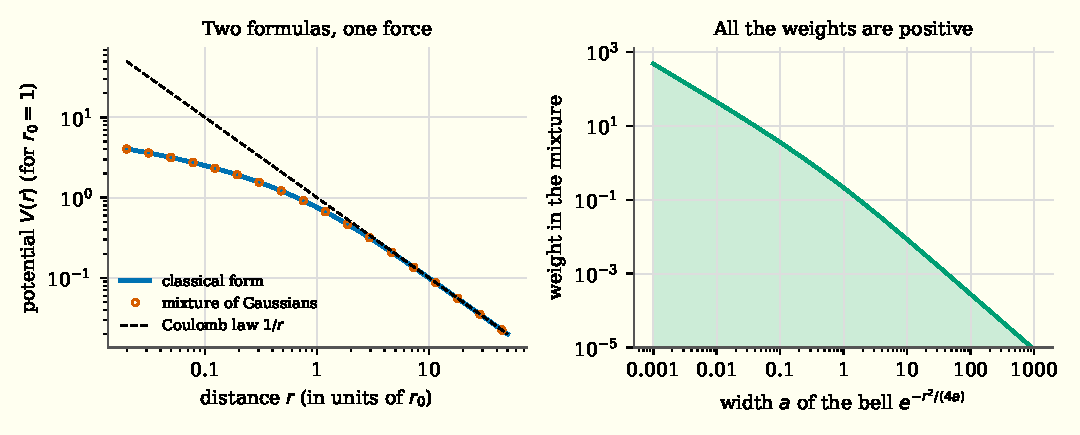
\includegraphics[width=\linewidth]{figures/c10_keldysh}
\caption{The classical formula and the pile of Gaussians coincide (left); the weights are all positive (right).}
\label{fig:c10}
\end{figure}

\section*{How we made sure it is not wrong}

In short: \niveau{C} for the identity ``it is a positive mixture of Gaussians'' (written proof, not checked by the machine), \niveau{A} for the
admissibility of the potential defined by this mixture and for the corollaries (conditional on the upstream
theorem), \niveau{X} for the computed energies.

For the Lean statements, ``the judge has looked'': the Lean kernel, the small program that checks every logical
step, accepted them with only three standard axioms, and the replay of 26 October 2026 passed them again without
error. At the stage of the article, producer and verifier were not separate; a distinct auditor, an AI agent, then
recompiled everything in its own directory and planted two false proofs (a hole, an invented axiom), both exposed.
It reran the Rust computation: result identical to the last bit.

Two episodes of this audit are worth telling. First, a sentence of the article, through a page-layout typo, read
``step~7 is not of level~C'', which inverted its own classification; it was corrected. Second, the auditor proposed
a simpler written proof, in which only positive quantities appear; it became the main proof, and it stays at
level~C, a line of reasoning carried out by AI agents, for lack of tools in the Lean library for these special functions. The register
remains marked ``unaudited'': no human has reread the statements.

\section*{What this does not say}

\begin{limite}
\begin{itemize}
\item The identity with the physical formula is a proof written on paper (\niveau{C}), not verified by the machine.
\item Since the force decreases like $1/r$, the sum over an infinite lattice diverges: the raw inequality must be
  read as ``infinity $\leq$ infinity'' and says nothing useful. For the softened version, the finiteness of the
  energy is not proved.
\item Everything is conditional on the upstream theorem, AI-generated and not peer reviewed.
\item The computed energies are static and classical, and compare only two lattices. The length $r_0$ of each
  material comes from the literature (\niveau{L}).
\item The novelty is modest: complete monotonicity follows quickly from textbook integrals.
\end{itemize}
\end{limite}

\section*{Going further}

The article, its register and the audit are deposited under doi:10.5281/\allowbreak zenodo.23646107. It is the
clearest example, in this book, of two levels of confidence kept separate within a single result.
